\documentclass{article}

\usepackage[utf8]{inputenc}
\usepackage{amsmath}
\usepackage{amsthm}
\usepackage{amssymb}
\usepackage[english]{babel}
\usepackage{graphicx}
\usepackage{setspace}
\usepackage[backend=bibtex,style=numeric,maxnames=10]{biblatex}
\usepackage[headsepline]{scrlayer-scrpage}
\usepackage{enumitem}
\usepackage{ulem}
\usepackage[table]{xcolor}
\usepackage{cleveref}
%\usepackage{listings}
%\usepackage{mathabx}
\usepackage{mathtools}
%\usepackage{textcomp}
%\usepackage{amsfonts}
%\usepackage{latexsym}
%\usepackage{eurofont}
%\usepackage[dvipsnames]{xcolor}
%\usepackage{caption}
%\usepackage{yfonts}
\usepackage{bbm}
\usepackage{algorithm}
\usepackage{algorithmic}
%\usepackage{paralist}
\usepackage{mathrsfs}
\usepackage{color}
%\usepackage{pdfpages}
\usepackage{arydshln}
\usepackage{graphicx}  % For including images
\usepackage{subcaption}  % For subfigures

%\lstset{
%    language=R,
%    keywordstyle=\color{blue},
%    commentstyle=\color{OliveGreen},
%    stringstyle=\color{BurntOrange},
%    breaklines=true
%}

\onehalfspacing
\parindent0mm

%\newtheorem{theorem}{Satz}[section]
\newtheorem{definition}{Definition}[section]
\newtheorem{proposition}{Proposition}[section]
%\newtheorem{lemma}{Lemma}[section]
%\newtheorem{corollary}{Korollar}[section]
\newtheorem{remark}{Remark}[section]
\newtheorem{example}{Example}[section]

\newcommand{\mc}[1]{{\mathcal#1}}
\newcommand{\E}{\mbox{I\negthinspace E}\,}
\newcommand{\indik}{\mathbbmss{1}}
\makeatletter
\newcommand*\bigcdot{\mathpalette\bigcdot@{.6}}
\newcommand*\bigcdot@[2]{\mathbin{\vcenter{\hbox{\scalebox{#2}{$\m@th#1\bullet$}}}}}
\newcommand{\bigbar}[1]{\mkern 1.5mu\overline{\mkern-1.5mu#1\mkern-1.5mu}\mkern 1.5mu}
\makeatother
\DeclareMathOperator{\sgn}{sgn}

\setlength{\textheight} {220mm}
\setlength{\textwidth} {150mm}

\setlength{\topmargin} {-20mm}
\setlength{\footskip} {25mm}

\setlength{\oddsidemargin} {10mm} 
\setlength{\marginparwidth} {0mm} 
\setlength{\marginparsep} {0mm}

\setcounter{secnumdepth}{4}
\setcounter{tocdepth}{4}
\setcounter{secnumdepth}{5}
\setcounter{tocdepth}{5}

\allowdisplaybreaks

\pagestyle{scrheadings}
\clearscrheadfoot
\automark{section}
\chead{\headmark}
\cfoot{\pagemark}

\begin{document}

\begin{titlepage}
\author{Marvin Zorn}

\begin{flushleft}
\vspace{200mm}
\end{flushleft}

\begin{center}
\huge
\textsc{A study on the logic game EggHead}\\

\end{center}

\normalsize

\vspace{170mm}

\center{Marvin Zorn}

\begin{center}
\textnormal{\today}
\end{center}

\end{titlepage}

\newpage

\tableofcontents

\newpage

\section{Introduction}

This document investigates the information theoretical aspects of "Egg Head," a logical card guessing game designed for three or more players. 

Players are rewarded points upon guessing their own cards correctly, first to score 10 wins. Guessing one's cards requires deductive reasoning based on information incrementally revealed. 

The paper proposes formulas on how players extract the necessary insights from logically structured questions and answers to address the challenge of concealed card deduction. However, the primary goal lies in analysing other players behaviour to gain even more information. The paper shows some simulation results based on a java application created over the last couple of years.

First, the game itself is explained, including a simplified example round. Based on that, the basic solving algorithm will be shown. In the fourth chapter, the core results will be derived, i.e. behavioural analysis formulae. Afterwards results are shown and the appendix finally contains some additional remarks.

\section{Game description}

\subsection{Overview}

Egg Head is a logical card guessing game playable by 3 or more players. 
The goal of the game is being the first one to determine one's own cards 10 times.
Each player is given a set of cards they must not see themselves. Instead, players can only see the cards of all other players.
The game is played by one player answering a random question about the cards they see, i.e. the cards of the other players. 
The answering player, called moderator, must answer truthfully.
Every other player can use the given answer to gain information about their own cards.
Since any of the other players and the moderator share common information about all other players cards, each player knows that only their own cards explain the "delta" between what they see and what the given answer implies.
Each round a new player becomes the moderator and a new random question is drawn.
As soon as someone solves, i.e. calls their cards, they are rewarded with a point if they guessed correctly. In any case, they receive a new set of cards and the game continues. 
The first player to collect 10 points wins.

\subsection{Setup}

EggHead contains two stacks of cards. One stack has cards with logical questions, the other has cards with values on them.
Values range from 1 to 6. Each card appears multiple times, for the sake of this analysis we assume that each card appears an infinite amount of times, so statistical deduction is out.

Each player is dealt 3 cards from the value-stack, which they place facing the other players, without looking at them.

\subsection{Round}

At the beginning of each round, the next-in-line player takes the moderator role for this round. 
The moderator draws one question and reads it aloud. Then they look at all the cards they see and answer the question truthfully.

All other players may use the information encapsulated in the answer to deduce information about their own cards.

After all players have made up their minds, the round is closed.

\subsection{Solving step}

At any time, a player can decide to call their cards. If they guessed correctly, they receive one point. Afterwards, they receive a new stack of 3 cards.

\subsection{End of the game}

The first player to gather 10 points wins.\footnote{Ties are possible, leading to more than player being winner}


\section{Basic deduction}

\subsection{Discussion of randomness and actions}

First thing to notice is that conditional on the realised questions and dealt card-stacks, the information flow is deterministic. 
There are no actual actions or strategies the player can choose to change the course of the game. 
Players have only one choice to make, which is solve or don't solve. 
Obviously, players could try to delude other players by behaving differently than they actually would based on the information they have collected. 
For the remainder we will assume that every player solves asap. 
This assumption removes choices alltogether, i.e. given a mechanism of deduction, each player is fully described.

\subsection{Information flow}

We can describe the state of a player as the list of valid combinations they still have to consider. With additional information, players can remove certain combinations. When only one combination is left, a player will solve.

For simplicity, the moderator will be a non-playing character, who simply answers the questions round after round. This only has minor impacts, for sake of completeness however, the formulas corresponding to a varying moderator among the players are given in the appendix.

\begin{example}\label{ex:Base}

Assume the following table:

\begin{tabular}{ccccc}
A & | & 1 & 2 & 2 \\
B & | & 4 & 5 & 6 \\
C & | & 3 & 3 & 3
\end{tabular}

The moderator draws the question: "How many numbers are missing?". The answer is "0". Player "A" instantly deduces that they must have at least one 1 and one 2. Therefore, player A can reduce their remaining valids to 

\begin{center}
\begin{tabular}{ccc}
1 & 2 & 1 \\
1 & 2 & 2 \\
1 & 2 & 3 \\
1 & 2 & 4 \\
1 & 2 & 5 \\
1 & 2 & 6
\end{tabular}
\end{center}

As soon as this list becomes monoelemental, A will solve.

\end{example}

\subsection{Putting together the maths}

Putting things in formulas we introduce the following notations:

\begin{definition}

Given $n$ players we call the set of players $P$ with $P = \{p_1, p_2, \ldots, p_n \}$ and define $I = \{1, \ldots, n\}$.

\end{definition}

\begin{definition}

We call the set of valids of one player $V_p$. Initially, the set consists of all card combinations a player can have. This set corresponds to an urn model with the configuration "With replacement, without order". The size of $V_p$ in a setup of 3-card stacks and 6 possible values per card is therefore given by $|V_p| = \left( \begin{array}{c}6+3-1 \\ 3 \end{array} \right) = 56$.

\end{definition}

\begin{definition}

$f: \left( \Omega^n, Q \right) \longrightarrow \mathbb{N}$ is called the answering function. It maps a set of stacks together with a question to the corresponding answer. Answers are typically numbers or booleans, with the latter encodable as 0 or 1. We can therefore use $\mathbb{N}$ as the image space.

\end{definition}

\begin{remark}\label{rem:AnswerAnalysis}

Given an answer $f_a$ to the question $q$, player $p_i$ will update their valids set as follows:

\begin{equation}
V_{p_i}^{posterior} = \{ v \in V_{p_i}^{prior} \, , \, f(s_1, \ldots, s_{i-1}, v, s_{i+1}, \ldots, s_n \, | \, q) = f_a \}
\label{Eq:q_a_base}
\end{equation}

where $s_j$ are the actual card stacks of the other players. The player assumes to have some combination $v$. They then check whether the hypothetical answer to the question would be the same as the actual answer. Keep only those $v$.

\end{remark}

\begin{example}

Recall \cref{ex:Base}. There we did intuitively, what we can now do mechanically. Let's rename the players to align to our new notation, $A = p_1, B = p_2, C = p_3$ and take the first entry of $V_{p_2}$ which may be $(1, 1, 1)$. Then we calculate $f$ as

\begin{eqnarray*}
f(s_{p_1}, v, s_{p_3} \, | \, q) &=& f((1, 2, 3), (1,1,1), (3, 4, 3) \, | \, q) \\
&=& 2
\end{eqnarray*}

Assuming $(1, 1, 1)$ for player $p_2$, the answer which the moderator need have given is 2. Therefore, $p_2$ can deduce not to have $(1, 1, 1)$. 

\end{example}

\cref{Eq:q_a_base} shows how to play the game perfectly based on the pure information received through the answer. Any human player who accomplishes this in their head (i.e. without taking notes on paper) can be congratulated. However, there is more...

\section{Behaviour analysis}

\subsection{Understanding the concept}

A player solves, if they have been able to deduce from the answers which cards they have. However, which information exactly a player can extract from an answer depends on the cards of the other players. Keeping a look out for the solving behaviour of the other players can therefore deliver additional insights.

\begin{example}\label{ex:3.3}

Recall \cref{ex:Base}:

\[
\begin{tabular}{ccccc}
$p_1$ & \vline & 1 & 2 & 2 \\
$p_2$ & \vline & 4 & 5 & 6 \\
$p_3$ & \vline & 3 & 3 & 3
\end{tabular} \]

Based on the answer (no numbers are missing), players can deduce the following valids:

\[
\begin{tabular}{ccccccccccc}
& $\underline{V_{p_1}}$ & & & & $\underline{V_{p_2}}$ & & & & $\underline{V_{p_3}}$ & \\
1 & 2 & 1 & & 4 & 5 & 6 & & 3 & x & y \\
1 & 2 & 2 \\
1 & 2 & 3 \\
1 & 2 & 4 \\
1 & 2 & 5 \\
1 & 2 & 6 \\
\end{tabular}
\]

where $(x,y) \in \{1,\ldots, 6\}^2 \, | \, x \leq y$. 

As already stated, $p_1$ can deduce to have at least one $1$ and one $2$. $p_2$ can solve immediately and $p_3$ can only deduce to have at least one $3$.

Next, $p_2$ will solve. This allows $p_1$ and $p_3$ to deduce to have neither 4, 5 or 6. \uline{Because if they had, $p_2$ would not have been able to solve.}

We end up with the following tables:

\[
\begin{tabular}{ccccccccccc}
& $\underline{V_{p_1}}$ & & & & $\underline{V_{p_2}}$ & & & & $\underline{V_{p_3}}$ & \\
1 & 2 & 1 & & 4 & 5 & 6 & & 3 & 1 & 1 \\
1 & 2 & 2 & &   &   &   & & 3 & 1 & 2 \\
1 & 2 & 3 & &   &   &   & & 3 & 1 & 3 \\
  &   &   & &   &   &   & & 3 & 2 & 2 \\
  &   &   & &   &   &   & & 3 & 2 & 3 \\
  &   &   & &   &   &   & & 3 & 3 & 3 \\
\end{tabular}
\]

What happened here? $p_1$ and $p_3$ performed a conditional analysis, checking which own cards would lead to which information gain for player $p_2$. We will formulate this in the following.

\end{example}

\begin{definition}

$\mathcal{V}_p: \bigtimes_{\hat{p} \in P \backslash p} \Omega \longrightarrow \mathcal{P}(\Omega)$ will be called the conditional Information. For each player, we collect in a scenario based way all combinations, which each other player could have and map this scenario to the valids list, the chosen player would then have constructed. That valids list will always be a set of elements of $\Omega$, therefore being some element of its power set.

\end{definition}

\begin{example}

Recall \cref{ex:Base} before any questions have been answered. $\mathcal{V}_{p_3}$ will look like this:

\begin{equation*}
\begin{array}{cccc}
p_1 & p_2 & \vline & p_3 \\ \hline
(1,1,1) & (1,1,1) & \vline & \{(1,1,1), (1,1,2), (1,1,6), \ldots, (6,6,6)\} \\
(1,1,1) & (1,1,2) & \vline & \{(1,1,1), (1,1,2), (1,1,6), \ldots, (6,6,6)\} \\
\vdots & \vdots & \vline & \vdots \\
(1,1,1) & \color{red} (4,5,6) & \vline & \{(1,1,1), (1,1,2), (1,1,6), \ldots, (6,6,6)\} \\
\vdots & \vdots & \vline & \vdots \\
(1,1,1) & (6,6,6) & \vline & \{(1,1,1), (1,1,2), (1,1,6), \ldots, (6,6,6)\} \\
(1,1,2) & (1,1,1) & \vline & \{(1,1,1), (1,1,2), (1,1,6), \ldots, (6,6,6)\} \\
\vdots & \vdots & \vline & \vdots \\
(1,1,2) & \color{red} (4,5,6) & \vline & \{(1,1,1), (1,1,2), (1,1,6), \ldots, (6,6,6)\} \\
\vdots & \vdots & \vline & \vdots \\
(1,1,2) & (6,6,6) & \vline & \{(1,1,1), (1,1,2), (1,1,6), \ldots, (6,6,6)\} \\
\vdots & \vdots & \vline & \vdots \\
\color{blue} (1,2,2) & (1,1,1) & \vline & \{(1,1,1), (1,1,2), (1,1,6), \ldots, (6,6,6)\} \\
\vdots & \vdots & \vline & \vdots \\
\color{blue} (1,2,2) & \color{red} (4,5,6) & \vline & \{(1,1,1), (1,1,2), (1,1,6), \ldots, (6,6,6)\} \\
\vdots & \vdots & \vline & \vdots \\
\color{blue} (1,2,2) & (6,6,6) & \vline & \{(1,1,1), (1,1,2), (1,1,6), \ldots, (6,6,6)\} \\
\vdots & \vdots & \vline & \vdots \\
(6,6,6) & (6,6,6) & \vline & \{(1,1,1), (1,1,2), (1,1,6), \ldots, (6,6,6)\} \\
\end{array} 
\end{equation*}

Note that each player can immediately filter all those rows, which they know are not correct. Player $p_1$ knows the cards of $p_2$, therefore they can filter to those rows, where the $p_2$ combination is correct and vice-versa. Remaining rows from $p_1$ perspective are colored red, from $p_2$ perspective are colored blue. The combination of both views reveals the single correct row, which is simultaneously the perspective of $p_3$ as the latter can see both player's cards. 

Now let's recreate the situation of \cref{ex:Base} and develop $\mathcal{V}_{p_3}$ accordingly. Question and answer have been "How many numberes are missing?" Answer: "0". Since the question is symmetric, all $\mathcal{V}_p$ will look alike, let's look at some example rows:

\[
\begin{array}{cccc}
p_1 & p_2 & \vline & p_3 \\ \hline
(1,1,1) & (1,1,1) & \vline & \{ \} \\
(1,1,1) & (1,1,2) & \vline & \{ \} \\
(1,2,3) & (4,5,1) & \vline & \{ (6,1,1), (6,1,2), \ldots, (6,1,6), (6,2,1), \ldots \} \\
(1,2,3) & (4,1,1) & \vline & \{ (5,6,1), (5,6,2), (5,6,3), (5,6,4), (5,6,5), (5,6,6) \} \\
(1,2,2) & (3,2,2) & \vline & \{ (4,5,6) \} \\
(1,2,2) & (3,3,3) & \vline & \{ (4,5,6) \} \\
(6,6,6) & (6,6,6) & \vline & \{ \}
\end{array} 
\]

In principle, this question and answer generates four scenarios\footnote{There is some mathematical background for this, i.e. linear equations}

\begin{itemize}
\item $(1,1,1), (1,1,1)$: Assuming these stacks for 2 players, the scenario is invalid. There is no stack which the third player could possibly have, to allow the given answer. We therefore remove all stacks from the set.
\item $(1,2,3), (4,5,1)$: In this scenario, the third player can deduce to have at least one $6$. All other cards are unknown.\footnote{There are corresponding scenarios in which the third player could deduce to have at least one $5$ etc. The same holds for the following bullet points}
\item $(1,2,3), (4,1,1)$: In this scenario, the third player can deduce to have at least one $5$ and one $6$.
\item $(1,2,2), (3,3,3)$: In this scenario, the third player can deduce to have exactly $(4,5,6)$.
\end{itemize}

Next, we ask all players for their reaction, i.e. solve or not solve. That reaction delivers information, which we will incorporate now.

There are two major steps to perform:

\begin{enumerate}
\item A player can either solve or not solve. The player will solve, if and only if, the length of the valids set is equal to 1. Otherwise, they will not solve. Therefore, for a given scenario, if the corresponding set of remaining valids does not align with the reaction, remove all entries of the set. Do this for all $\mathcal{V}_p$. As a result, we end up with the two different variants:

Player solved:
\[
\begin{array}{cccc}
p_1 & p_2 & \vline & p_3 \\ \hline
(1,1,1) & (1,1,1) & \vline & \{ \} \\
(1,1,1) & (1,1,2) & \vline & \{ \} \\
(1,2,3) & (4,5,1) & \vline & \color{green} \{ \} \color{black} \\
(1,2,3) & (4,1,1) & \vline & \color{green} \{ \} \color{black} \\
(1,2,2) & (3,2,2) & \vline & \{ (4,5,6) \} \\
(1,2,2) & (3,3,3) & \vline & \{ (4,5,6) \} \\
(6,6,6) & (6,6,6) & \vline & \{ \}
\end{array} 
\]

Player didn't solve:
\[
\begin{array}{cccc}
p_1 & p_2 & \vline & p_3 \\ \hline
(1,1,1) & (1,1,1) & \vline & \{ \} \\
(1,1,1) & (1,1,2) & \vline & \{ \} \\
(1,2,3) & (4,5,1) & \vline & \{ (6,1,1), (6,1,2), \ldots, (6,1,6), (6,2,1), \ldots \} \\
(1,2,3) & (4,1,1) & \vline & \{ (5,6,1), (5,6,2), (5,6,3), (5,6,4), (5,6,5), (5,6,6) \} \\
(1,2,2) & (3,2,2) & \vline & \color{green} \{ \} \color{black} \\
(1,2,2) & (3,3,3) & \vline & \color{green} \{ \} \color{black} \\
(6,6,6) & (6,6,6) & \vline & \{ \}
\end{array} 
\]

\item The next insight we can gain is to check which valids of a given set are possible according to the remaining tables. Back in \cref{ex:3.3} we removed several combinations of $p_3$s valids list, based on the solving behaviour of $p_2$. Why has $p_3$ been able to remove, e.g. (3,1,4) from their valids set? The row in $\mathcal{V}_{p_3}$ is 

\[
\begin{array}{cccc}
p_1 & p_2 & \vline & p_3 \\ \hline
(1,2,2) & (4,5,6) & \vline & \{(3,1,1), (3,1,2), (3,1,3), (3,1,4) \ldots,  (3,6,6) \\
\end{array}
\]

Now we check whether $(3,1,4)$ is a valid combination according to the other tables. The corresponding row in $\mathcal{V}_{p_1}$ is

\[
\begin{array}{cccc}
p_3 & p_2 & \vline & p_1 \\ \hline
(3,1,4) & (4,5,6) & \vline & \{ (2,1,1), \ldots, (2,2,1), \ldots, (2,6,6) \}
\end{array}
\]

Since $p_1$ did not solve, this scenario is possible. Next, we check the table $\mathcal{V}_{p_2}$. The row (after application of step 1) is

\[
\begin{array}{cccc}
p_1 & p_3 & \vline & p_2 \\ \hline
(1,2,2) & (3,1,4) & \vline & \{ \}
\end{array}
\]

This scenario has become impossible due to step 1. (3,1,4) can therefore be excluded from the corresponding valids list of $\mathcal{V}_{p_3}$. Note that this must be done for every valid in every row separately, i.e. (3,1,4) cannot simply be removed from all rows in $\mathcal{V}_{p_3}$.
 
\end{enumerate}

\end{example}

The conditional Information shows which valids a player would have, given a scenario set of stacks for the other players. Given such a scenario, anyone can deduce the valids, which the remaining player would have. Therefore the conditional Information is public information and everyone can use every table. However, we need to ensure that the tables are updated in such a way, which uphold this property. We have already incorporated the question/answer step as well as the solving behaviour step. Both informations are public, therefore incorporating them upholds public property of $\mathcal{V}_p$. We will put this into formulas and finally, we need to perform some kind of reset, whenever one or multiple players solve. 

\subsection{Updating conditional Information based on q/a and reactions}

\begin{remark}\label{re:BehaviourAnalysis}

The conditional Information $\mathcal{V}_p$ is initialized by creating one table for each player. Each table maps every combination of stacks, which the other players can have onto an element of $\mathcal{P}(\Omega)$. $\mathcal{V}_p$ will be updated during the course of the game. In the following, we will consider $i \in I$ and define $J := I \backslash i$.

Question/Answer step:

Assume a question $q \in Q$ and an answer $f_a$. Then\footnote{The formula is the same as \cref{Eq:q_a_base}}

\begin{equation}
\mathcal{V}_{p_i}^{posterior}(\bigtimes_{j \in J} \, s_{p_j}) = \{ v \in \mathcal{V}_{p_i}^{prior}(\bigtimes_{j \in J} \, s_{p_j}) \, | \, f(\bigtimes_{j \in J} s_{p_j} \times v \, | \, q) = f_a \}
\label{Eq:q_a}
\end{equation}

Behavioural step:

Assume reactions $r_p \in \{0, 1 \} \, , \, p \in P$, where $r=1$ means solve and $r=0$ means don't solve. Then

\begin{equation}
\mathcal{V}_{p_i}^{posterior}(\bigtimes_{j \in J} \, s_{p_j}) = \left \{ 
								 \begin{array}{ccc} 
																	 \mathcal{V}_{p_i}^{prior}(\bigtimes_{j \in J} \, s_{p_j}) & ; & \indik_{|\hat{V}| = 1} = r_p \\
																	 \{\} & ; & else
								 \end{array} \right.
\label{Eq:react_1}
\end{equation}

where $\hat{V} := \mathcal{V}_{p_i}^{prior}(\bigtimes_{j \in J} \, s_{p_j})$ is a short hand notation for the currently investigated row of $\mathcal{V}_p$. Keep the valids list only for those rows, where the current valids list fits the reaction. Do this for all players first.

Next,

\begin{equation}
\mathcal{V}_{p_i}^{posterior}(\bigtimes_{j \in J} \, s_{p_j}) = \{ v \in \hat{V} \, | \, s_{p_k} \in \mathcal{V}_{p_k}^{prior}(\bigtimes_{j \in J \backslash k} \, s_{p_j}, v) \, \forall \, k \in J \}
\label{Eq:react_2}
\end{equation}

Cross reference a valid from one row into all the other tables, each time taking the valid together with the row-specific combinations for the other players, except the player of the currently cross-referenced table. Check whether the row-specific combination of that player is part of the respective valids list.

Note that after the application of the behavioural analysis tables have changed. We therefore need to ask every player for a new reaction based on their updated information status and repeat the process. We do this until no table is updated anymore. Afterwards we can close the round.

\end{remark}

\subsection{Updating conditional Information after a solving step}

When a player solves, they receive a new stack. Obviously, their associated table needs to be simply reset. However, what happens to the other tables? We will look at \cref{ex:Base} to illustrate.

\begin{example}

Recall \cref{ex:Base}. Player $p_2$ solved after one round. What happens to the tables of the other two players, while keeping the necessity of upholding public availability in mind. Well, player $p_2$ knows their own cards now, so they can go into both other tables and identify the exact row, which corresponds to reality. Therefore, $p_2$ has now complete information about the current state of the game. $p_1$ on the other hand does not have this information about $p_3$. They can still only identify the correct block, by fixing the correct stack of $p_2$. But since $p_2$ will receive new cards now, all combinations are possible again. So what we simply do, is to duplicate each row in the table, where the combination of $p_2$ is correct, and create new rows with all possible combinations.

\[
\begin{array}{cccc}
p_1 & p_2 & \vline & p_3 \\ \hline
\color{red} (1,1,1) & \color{red} (1,1,1) & \vline & \color{red} \{ \} \\
\color{green} (1,1,1) & \color{green} (4,5,6) & \vline & \color{green} \{ (2,3,1), (2,3,2), (2,3,3), (2,3,4), (2,3,5), (2,3,6) \} \\  \hdashline

\color{red} (2,2,1) & \color{red} (2,3,4) & \vline & \color{red} \{ (5,6,1), (5,6,2), (5,6,3), (5,6,4), (5,6,5), (5,6,6) \} \\
\color{red} (2,2,1) & \color{red} (3,4,5) & \vline & \color{red} \{ (6,1,1), (6,1,2), \ldots, (6,1,6), (6,2,1), \ldots \} \\
\color{green} (2,2,1) & \color{green} (4,5,6) & \vline & \color{green} \{ (3,1,1), (3,1,2), \ldots, (3,1,6), (3,2,1), \ldots \} \color{black} \\  \hdashline

\color{red} (2,2,2) & \color{red} (1,2,4) & \vline & \color{red} \{ (3,5,6) \} \\
\color{green} (2,2,2) & \color{green} (4,5,6) & \vline & \color{green} \{ (1,3,1), (1,3,2), (1,3,3), (1,3,4), (1,3,5), (1,3,6) \} \color{black} \\  
\end{array} 
\]

Becomes

\[
\begin{array}{cccc}
p_1 & p_2 & \vline & p_3 \\ \hline
(1,1,1) & (1,1,1) & \vline & \{ (2,3,1), (2,3,2), (2,3,3), (2,3,4), (2,3,5), (2,3,6) \} \\
(1,1,1) & (4,5,6) & \vline & \{ (2,3,1), (2,3,2), (2,3,3), (2,3,4), (2,3,5), (2,3,6) \} \\  \hdashline

(2,2,1) & (2,3,4) & \vline & \{ (3,1,1), (3,1,2), \ldots, (3,1,6), (3,2,1), \ldots \} \\
(2,2,1) & (3,4,5) & \vline & \{ (3,1,1), (3,1,2), \ldots, (3,1,6), (3,2,1), \ldots \} \\
(2,2,1) & (4,5,6) & \vline & \{ (3,1,1), (3,1,2), \ldots, (3,1,6), (3,2,1), \ldots \} \\  \hdashline

(2,2,2) & (1,2,4) & \vline & \{ (1,3,1), (1,3,2), (1,3,3), (1,3,4), (1,3,5), (1,3,6) \} \\
(2,2,2) & (4,5,6) & \vline & \{ (1,3,1), (1,3,2), (1,3,3), (1,3,4), (1,3,5), (1,3,6) \} \\  
\end{array} 
\]

\end{example}

\begin{remark}\label{rem:reset}

Assume player $p_k$ solved with solution $\mathbf{s}_k$. Perform the following steps to accurately reflect this in the conditional information tables.

\begin{enumerate}
\item Reset $\mathcal{V}_{p_k}$
\item For each $p_i \, , \, i \neq k$ do: 
\begin{equation} 
\mathcal{V}_{p_i}^{posterior}(\bigtimes_{j \in J} s_j) = \mathcal{V}_{p_i}^{prior}(\bigtimes_{j \in J \backslash k} s_j \times \mathbf{s}_k) 
\label{Eq:reset}
\end{equation}
For a given row, we lookup the correct row and duplicate its valids list.
\end{enumerate}

\end{remark}

\newpage

\subsection{Algorithmic depiction}

\begin{remark}

Outline of the full algorithm:

\begin{algorithm}
\caption{Playing EggHead using behavioural analysis}
\label{alg:game_process}
\begin{algorithmic}[1]
\WHILE{no player has achieved 10 points}
    \STATE Draw question and answer it
    \STATE Apply \cref{Eq:q_a}
    \REPEAT
        \STATE Show the reactions (extract from the appropriate row in the conditional information tables)
        \STATE Apply \cref{Eq:react_1} for all tables in arbitrary order
        \STATE Apply formula \cref{Eq:react_2} for all tables in arbitrary order
        \IF{someone solved}
            \STATE Apply formula \cref{Eq:reset} in arbitrary order
        \ENDIF
    \UNTIL{no update happened}
\ENDWHILE
\end{algorithmic}
\end{algorithm}

\end{remark}

Algorithm 1 is the key result of this paper. It has been implemented in java to perform a couple simulations. The results are shown in the following chapter.

\section{Results}

Setup: External moderator, 23 logical questions, 6 possible values per card, 4 players, 3 cards per player. 

Behavioural analysis will be abbreviated with BA.

Simulated were games with 1000 rounds (removing the score cap of 10 points). Collected were the number of rounds needed to solve, with the counter resetting after a solve step. So having $p_1$ use BA and the three others not use BA we can treat the counts of player $p_1$ as observations of the random variable $X=$ \textit{How many rounds are needed to solve}. The counts for the other players are assumed to be equally distributed and independent and therefore collected in a single observations list.
The empirical cumulative distribution function for both modes are shown below. Next, based on this CDF, the CDF for scoring 10 points has been calculated using convolution. The results are displayed below.
    
\begin{figure}[H]
    \centering
    \begin{subfigure}{0.45\textwidth}
        \centering
        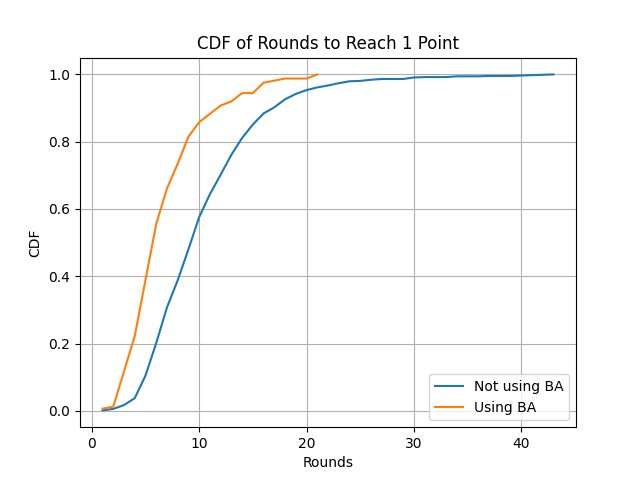
\includegraphics[width=\linewidth]{cdf_rounds_to_score_1.png}
        \caption{Empirical CDF of rounds needed to score 1 point}
    \end{subfigure}
    \hfill
    \begin{subfigure}{0.45\textwidth}
        \centering
        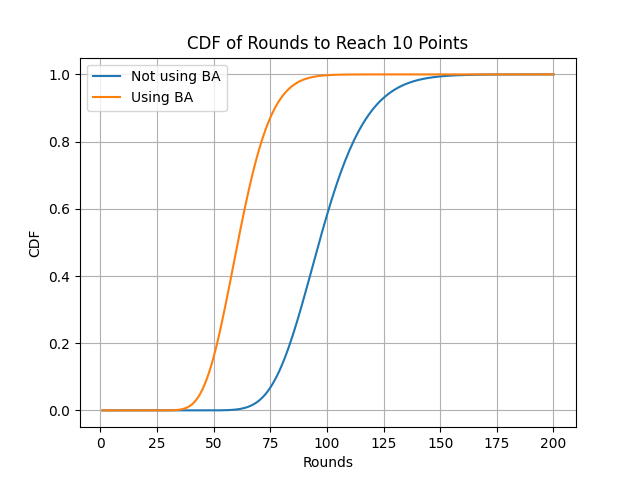
\includegraphics[width=\linewidth]{cdf_rounds_to_score_10.png}
        \caption{Empirical CDF of rounds needed to score 10 points}
    \end{subfigure}

    \caption{CDFs of rounds needed for scoring 1 or 10 points per mode}
    \label{fig:cdf_rounds}
\end{figure}

As expected, using BA results in significantly less rounds required to solve. Additional key figures are shown in below table.

\begin{center}
\begin{tabular}{c|cc}
\centering
\textbf{Mode} & \textbf{Mean} & \textbf{Variance} \\
Not using BA & 9.78 & 29.3 \\
Using BA & 6.16 & 14
\end{tabular}
\end{center}

Next, the dependency on the required rounds to score on the amount of players actually using BA is investigated. Results are shown in \cref{fig:cdf_multiple}.

\begin{figure}[H]
    \centering
    \begin{subfigure}{0.45\textwidth}
        \centering
        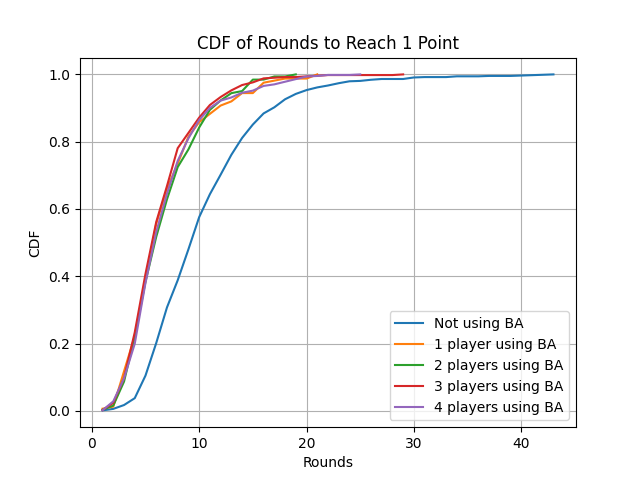
\includegraphics[width=\linewidth]{cdf_rounds_to_score_1_per_playermode.png}
        \caption{Empirical CDF of rounds needed to score 1 point}
    \end{subfigure}
    \hfill
    \begin{subfigure}{0.45\textwidth}
        \centering
        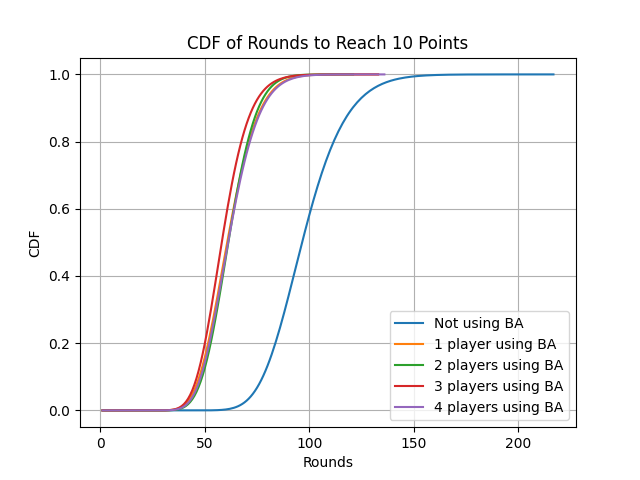
\includegraphics[width=\linewidth]{cdf_rounds_to_score_10_per_playermode.png}
        \caption{Empirical CDF of rounds needed to score 10 points}
    \end{subfigure}

    \caption{CDFs of rounds needed for scoring 1 or 10 points with multiple players using BA} 
    \label{fig:cdf_multiple}
\end{figure}

The number of players utilizing BA does not seem to have an impact on the rounds required, the cdfs are all close and intersecting. This suggests that, despite the pace of the game increasing with the amount of players using BA, as solves happen more frequent, this effect does not cumulate.

Last, the winning probabilities have been simulated based on the above CDFs. Results are shown in \cref{Fig:winning_prob}.\footnote{The total sum of probabilities exceeds 100\% due to ties}

\begin{figure}[H]
    \centering
    % First row
    \begin{subfigure}{0.45\textwidth}
        \centering
        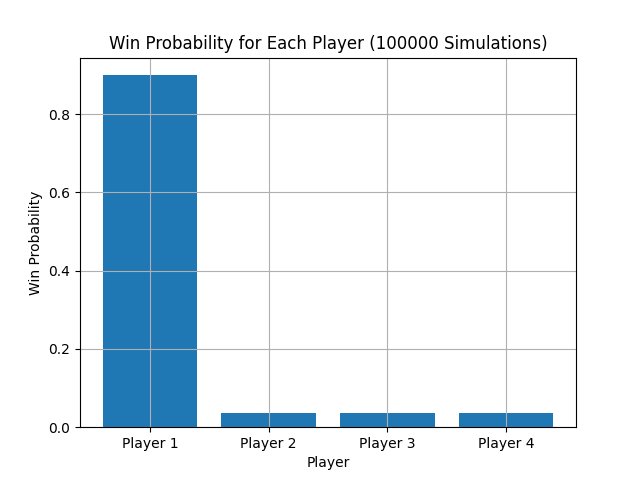
\includegraphics[width=\linewidth]{winning_probabilities_per_mode_1.png}
        \caption{Player 1 using BA}
    \end{subfigure}
    \hfill
    \begin{subfigure}{0.45\textwidth}
        \centering
        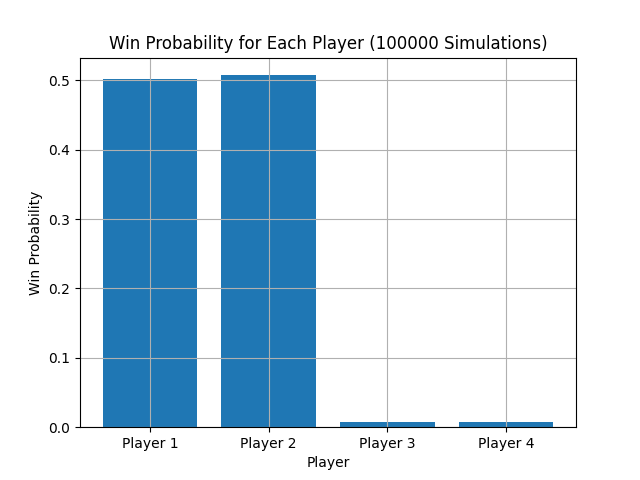
\includegraphics[width=\linewidth]{winning_probabilities_per_mode_2.png}
        \caption{Player 1-2 using BA}
    \end{subfigure}
    
    % Second row
    \begin{subfigure}{0.45\textwidth}
        \centering
        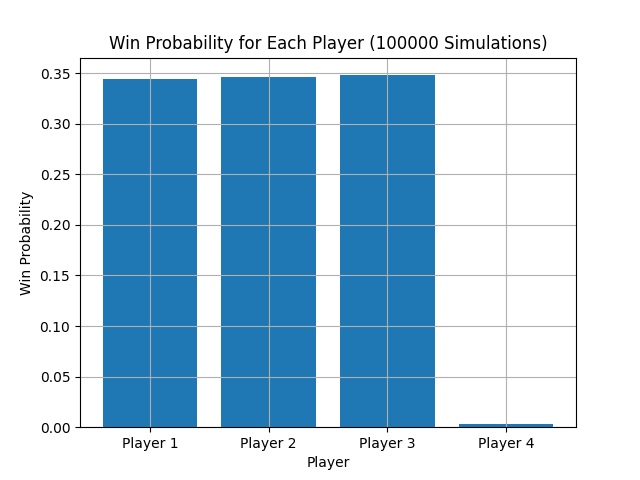
\includegraphics[width=\linewidth]{winning_probabilities_per_mode_3.png}
        \caption{Player 1-3 using BA}
    \end{subfigure}
    \hfill
    \begin{subfigure}{0.45\textwidth}
        \centering
        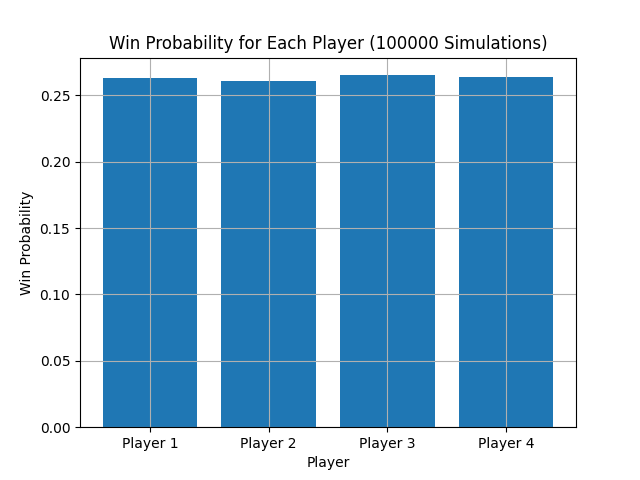
\includegraphics[width=\linewidth]{winning_probabilities_per_mode_4.png}
        \caption{Player 1-4 using BA}
    \end{subfigure}

    \caption{winning probabilities per player}
    \label{Fig:winning_prob}
\end{figure}

It is quite obvious that utilizing BA leads to almost 100\% chance of winning the game, given no other player uses BA. Indeed, whenever multiple players utilize BA, they share the chance of winning evenly, leaving almost no chance for the others. 

\newpage
\appendix
\section{Appendix}

\subsection{Master Table}

The conditional information table for player $p_i$ contains, per combination of cards stack of the other players, the valids list of $p_i$ conditional of those other cards stacks being actual reality. However, in principle we can collect all valid combinations in a single table. 

\begin{definition}

$V_M : \bigtimes_{p \in P} \Omega \longrightarrow \Omega$ will be called master table. Initially, it contains all possible  combinations of cards, i.e. any combinations of cards any player could have in all imaginable combinations.

\end{definition}

\begin{remark}

We have already calculated the amount of initially possible combinations per player. Calculating the state space of $V_M$ is straightforward, since it corresponds to an urn model with the configuration "With replacement, with order". The state space is therefore  $|V|^{|P|}$, i.e. the amount of combinations per player to the power of amount of players. 3-card stacks, 6 possible values per card and 4 players lead to $56^4 = 9.8$ mn.

\end{remark}

\begin{example}

Let's assume we have 3 players and cards range from 1 to 6. Then, $V_{M}$ will look like this:

\begin{equation*}
\begin{array}{ccc}
p_1 & p_2 & p_3 \\ \hline
(1,1,1) & (1,1,1) & (1,1,1) \\
(1,1,1) & (1,1,1) & (1,1,2) \\
\vdots & \vdots & \vdots \\
(1,1,1) & (1,1,1) & (1,1,6) \\
\vdots & \vdots & \vdots \\
(1,1,1) & (1,1,1) & (6,6,6) \\
(1,1,1) & (1,1,2) & (1,1,1) \\
\vdots & \vdots & \vdots \\
(1,1,1) & (1,1,2) & (6,6,6) \\
\vdots & \vdots & \vdots \\
(1,1,1) & (6,6,6) & (6,6,6) \\
\vdots & \vdots & \vdots \\
(6,6,6) & (6,6,6) & (6,6,6)
\end{array} 
\end{equation*}

\end{example}

\begin{remark}

The master table aims at collecting the publicly available information, i.e. which stack combinations are still possible, from at least one persons perspective. Keep in mind, that for $p_1$ to make deductions from $p_2$ behaviour, $p_1$ must know what $p_2$ knows. Let us look at two examples to illustrate the difference: Consider these hands: $p_1 = (1,2,2) \, , \, p_2 = (4,5,6) \, , \, p_3 = (3,3,3)$. All players can immediately deduce that both $(6,6,6), (6,6,6), (6,6,6)$ and $(6,6,6), (4,5,6), (6,6,6)$ are invalid. However, for the first combination, each player also knows, that each other player can invalidate it. $p_1$ knows that $p_2$ sees (3,3,3) on $p_3$ hand. $p_1$ therefore also knows, that $p_2$ can invalidate the combination. Now consider the second combination. $p_1$ can invalidate it, because $p_3$ doesn't have (6,6,6). In fact, $p_3$ can also invalidate it, because $p_1$ neither has (6,6,6). But both of them don't know that the other can invalidate the scenario. That is because $p_1$ doesn't know their own cards. They may have (6,6,6) and if they had, $p_3$ would keep the combination in their valids list, as from their perspective, they could have (6,6,6) themselves, too. This combination can therefore not be removed from the master table, as there is at least one player, who doesn't know whether all other players can invalidate the row. 

\end{remark}

\begin{remark}

The master table and the conditional information tables contain the same information. The conditional information tables are projections of the master table onto a single player, basically they are a "groupby" statement.

\[ \mathcal{V}_{p_i}(\bigtimes_{j \in J} s_j) = \{ v \in \Omega \, | \, \bigtimes_{j \in J} s_j \times v \in V_M \} \]

\end{remark}

\begin{example}

Assume the following master table:

\begin{equation*}
\begin{array}{ccc}
p_1 & p_2 & p_3 \\ \hline
(1,1,1) & (4,5,6) & (3,3,3) \\
(1,2,1) & (4,5,6) & (3,3,3) \\
(1,2,2) & (1,1,1) & (3,3,3) \\
(1,2,2) & (4,5,6) & (1,1,1) \\
(1,2,2) & (4,5,6) & (6,6,6) \\
(1,2,2) & (6,6,6) & (3,3,3) \\
(6,6,6) & (4,5,6) & (3,3,3)
\end{array} 
\end{equation*}

Then the corresponding conditional information tables will look like this:

\[ \left. \mathcal{V}_{p_1} = \right. 
\begin{array}{cccc}
p_2 & p_3 & \vline & p_1 \\ \hline
(4,5,6) & (3,3,3) & \vline & (1,1,1), (1,2,1) \\
(1,1,1) & (3,3,3) & \vline & (1,2,2) \\
(4,5,6) & (1,1,1) & \vline & (1,2,2) \\
(4,5,6) & (6,6,6) & \vline & (1,2,2) \\
(6,6,6) & (3,3,3) & \vline & (1,2,2) \\
(4,5,6) & (3,3,3) & \vline & (6,6,6)
\end{array} 
\]

\[ \left. \mathcal{V}_{p_2} = \right. 
\begin{array}{cccc}
p_1 & p_3 & \vline & p_2 \\ \hline
(1,1,1) & (3,3,3) & \vline & (4,5,6) \\
(1,2,1) & (3,3,3) & \vline & (4,5,6) \\
(1,2,2) & (3,3,3) & \vline & (1,1,1),(6,6,6) \\
(1,2,2) & (1,1,1) & \vline & (4,5,6) \\
(1,2,2) & (6,6,6) & \vline & (4,5,6) \\
(6,6,6) & (3,3,3) & \vline & (4,5,6)
\end{array} 
\]

\[ \left. \mathcal{V}_{p_3} = \right. 
\begin{array}{cccc}
p_1 & p_2 & \vline & p_3 \\ \hline
(1,1,1) & (4,5,6) & \vline & (3,3,3) \\
(1,2,1) & (4,5,6) & \vline & (3,3,3) \\
(1,2,2) & (1,1,1) & \vline & (3,3,3) \\
(1,2,2) & (4,5,6) & \vline & (1,1,1), (6,6,6) \\
(1,2,2) & (6,6,6) & \vline & (3,3,3) \\
(6,6,6) & (4,5,6) & \vline & (3,3,3)
\end{array} 
\]

In fact, each conditional information table holds the same information and can be flattened into the master table. However, the conditional information tables store the information in a more efficient way, when it comes to implementation and computational time.

\end{example}

%\begin{example}
%
%Given the hands $p_1 = (1,2,2) \, , \, p_2 = (4,5,6) \, , \, p_3 = (3,3,3)$ the table immediately reduces to
%
%\begin{equation*}
%\begin{array}{ccc}
%p_1 & p_2 & p_3 \\ \hline
%(1,1,1) & (4,5,6) & (3,3,3) \\
%\vdots & \vdots & \vdots \\
%(1,2,1) & (4,5,6) & (3,3,3) \\
%(1,2,2) & (1,1,1) & (3,3,3) \\
%(1,2,2) & (4,5,6) & (1,1,1) \\
%\vdots & \vdots & \vdots \\
%(1,2,2) & (4,5,6) & (6,6,6) \\
%(1,2,2) & (6,6,6) & (3,3,3) \\
%\vdots & \vdots & \vdots \\
%(6,6,6) & (4,5,6) & (3,3,3)
%\end{array} 
%\end{equation*}
%
%from $p_3$ perspective, (6,6,6), (4,5,6), (6,6,6) is a combination that $p_1$ might see as possible. Even though $p_3$ knows its wrong. The other way round works as well. 
%Perhaps keep rows where up to 2 stacks are wrong. The corresponding players do not know that the other player can remove it. Whereas the row (6,6,6), (6,6,6), (6,6,6) can be removed, as all players know that every other player also knows it to be wrong.
%
%Further thoughts: Given (1,1,1), (2,2,2), (3,3,3), everyone can deduce that 3x(6,6,6) is not possible. Furthermore, everyone knows for everyone else that they know, too. For the reason above ($p_1$ sees $p_3$ and knows $p_2$ does too). However, $p_1$ does not know that $p_2$ knows that $p_3$ can invalidate the combination. Because what $p_2$ uses for that deduction is what they see on $p_1$ hand, which $p_1$ doesn't know. Assuming $p_1$ had (6,6,6), $p_2$ would actually not know that $p_3$ can invalidate 3x(6,6,6). So by saying: Hey everyone, I know that you all know that 3x(6,6,6) is not possible, so let us remove it from the master table, you give away that neither of the other two have (6,6,6) on their hands. Because if they did, you hadn't been able to come up with that deduction. 
%
%\textbf{That means, we cannot remove combinations from the Scenario table based on what everyone sees on each others hands, at all. Updates may only happen based on q/a and reactions. Personal deductions must then be based on querying the table.}
%
%keep in mind that due to ordering ambiguity, we need to loop updatebyReaction until convergence. And then ask players again, if something changed, so an outer loop for convergence
%
%\end{example}

\subsection{Variants}

\begin{remark} Varying moderator

If the moderator role rotates along the players, the formulas need almost no adjustments. In \cref{Eq:q_a} the condition will always remove the current moderator from the cross-product:

\begin{equation}
\mathcal{V}_{p_i}^{posterior}(\bigtimes_{j \in J} \, s_{p_j}) = \{ v \in \mathcal{V}_{p_i}^{prior}(\bigtimes_{j \in J} \, s_{p_j}) \, | \, f(\bigtimes_{j \in J \backslash \, m} s_{p_j} \times v \, | \, q) = f_a \}
\end{equation}

where $m$ is the index of the current moderator.

\cref{Eq:react_1} will only be applied to the non-moderator players.

\end{remark}

\begin{remark} Partial behavioural analysis

If not all players perform the behavioural analysis, but only a subset, then steps 7 and 9 of algorithm 1 are only executed for the tables of those players who do perform the analysis. Note that step 6 is still necessary for all players, since it incorporates the reaction of a player into their respective conditional information table which is then used by the analysing players. Of course, if no player performs behavioural analysis, the entire loop is omitted. 

\end{remark}

\end{document}